\section{La répartition des médecins}

\subsection{Actifs et retraités actifs}

Le diagramme de la figure \ref{fig:repartition} donne la répartition des médecins actifs inscrits au conseil de l'ordre en 2011.

\begin{figure}{h}
	\begin{center}
		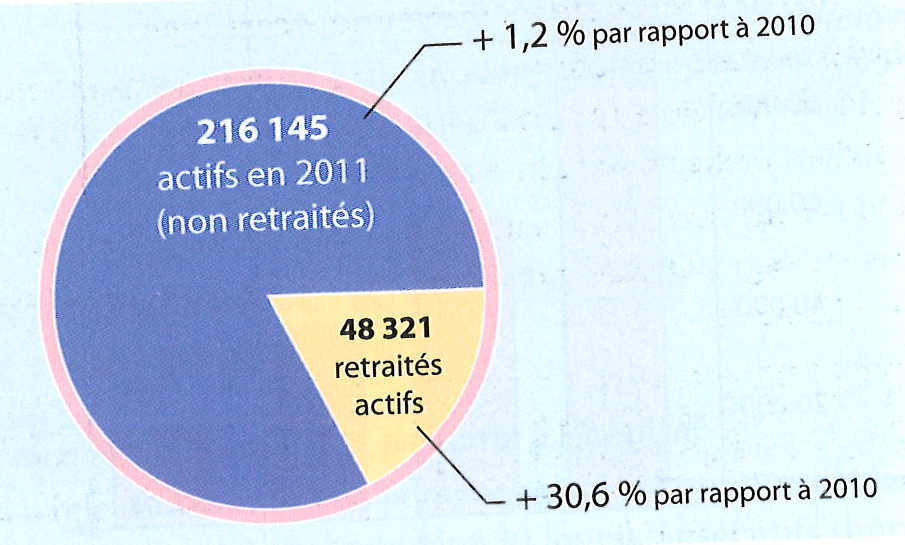
\includegraphics[scale=0.8]{repartition}
		\caption{Répartition des médecins actifs en 2011}
		\label{fig:repartition}
	\end{center}
\end{figure}


\begin{questions}
	\question Quel pourcentage de l'ensemble des médecins actifs représentent les médecins retraités en 2011 ? Arrondir à \num{0.1} \%.
	
	\question Déterminer le nombre de médecins actifs non retraités en 2010.
	
	\question Déterminer le nombre de médecins actifs retraités en 2010.
	
	\question Déterminer l'augmentation en pourcentage du nombre de médecins actifs entre 2010 et 2011. Arrondir à \num{0.1} \%.
	
\end{questions}

\subsection{Les modes d'exercice}

\begin{questions}
	
	\question Le diagramme de la figure \ref{fig:mode_exercice1} donne la répartition des modes d'exercice des médecins actifs inscrits au conseil de l'ordre en 2011. Déterminer l'effectif pour chacun des modes d'exercice.
	
	\begin{figure}{h}
		\begin{center}
			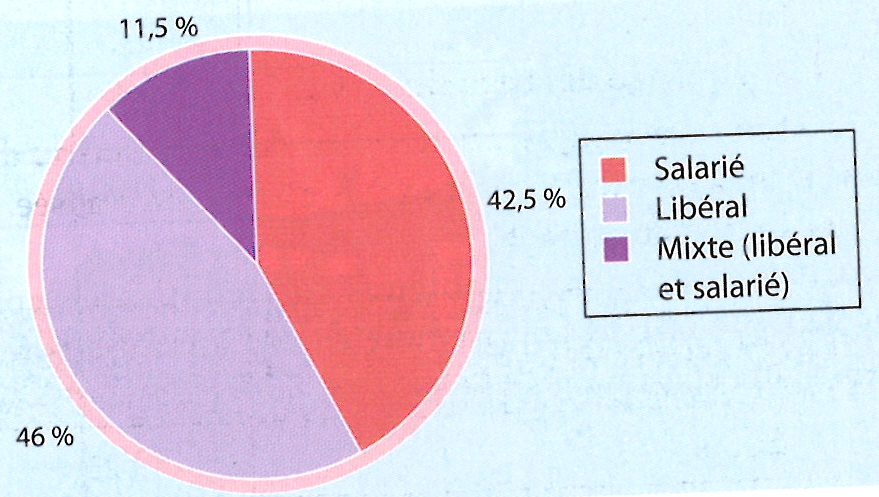
\includegraphics[scale=0.4]{mode_exercice1}
			\caption{Modes d'exercice des médecins actifs en 2011}
			\label{fig:mode_exercice1}
		\end{center}
	\end{figure}
	
	\question Le diagramme de la figure \ref{fig:mode_exercice1} donne la répartition des modes d'exercice des \num{27774} médecins de moins de 40 ans en 2011. Donner l'effectif pour chacun des modes d'exercice.
	
	\begin{figure}{h}
		\begin{center}
			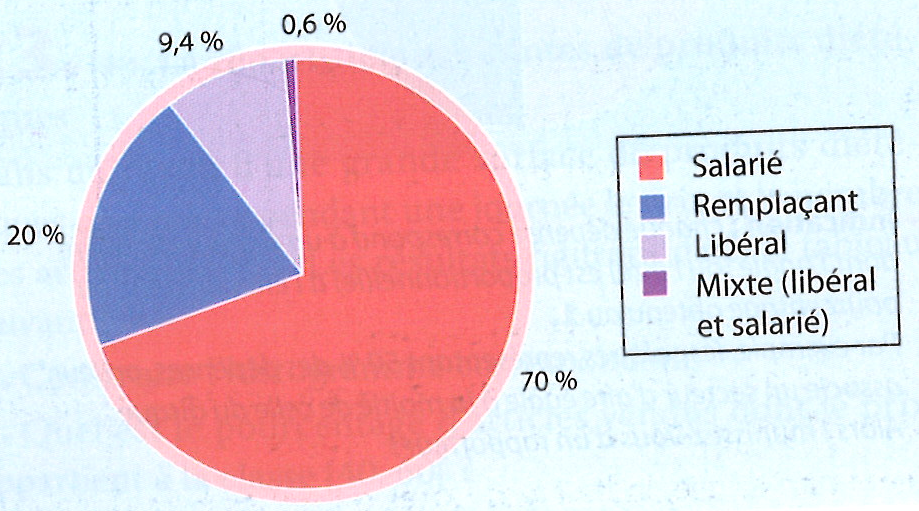
\includegraphics[scale=0.4]{mode_exercice2}
			\caption{Modes d'exercice des moins de 40 ans en 2011}
			\label{fig:mode_exercice2}
		\end{center}
	\end{figure}
	
	
	\question Quel commentaire peut-on faire sur les modes d'exercice des médecins actifs ?
\end{questions}